\section{Results}
\label{sec:results}

\subsection{Response to input resolution}
\label{sec:response}

We begin with the most direct question: what happens to accuracy when every view is made larger or smaller? If more pixels simply meant more information, accuracy should rise and then saturate for both models. \Cref{fig:response} shows pose accuracy when all 12 views of a scene are resized to one size, on ETH3D and HiRoom.

\paragraph{VGGT has a narrow optimum.}
On both datasets VGGT is most accurate at a width of 504\,px, the tested size closest to the 518\,px it uses by default, where it reaches 23.1 \auc on ETH3D and 45.5 on HiRoom. Larger inputs make it worse even though they contain more detail: at 588--630\,px it loses 31--60\% of that accuracy, and the step from 546 to 630\,px alone costs 11.8 \auc on ETH3D \ci{-19.8}{-5.3} and 22.0 on HiRoom \ci{-28.3}{-15.5}, with the larger input better in 0 of 8 and 1 of 19 scenes. Smaller inputs cost more: at 392--448\,px VGGT loses 54--76\% of its best accuracy. VGGT therefore works well only in a narrow band of input sizes around the one it uses by default.

\paragraph{\pithree improves and then levels off.}
\pithree gains accuracy as the input grows and then stops gaining, without a significant decline in the range we tested. Where it levels off depends on the dataset. On ETH3D, it rises from 13.3 \auc at 224\,px to 28.5 at 322\,px and then stays between 26.3 and 29.3 up to 630\,px; for example, 546\,px is no better than 448\,px ($-0.1$ \ci{-1.8}{1.4}). On HiRoom it keeps improving for longer, from 27.9 at 182\,px to 57.1 at 364\,px and 63.4 at 546\,px ($+6.3$ over 364\,px, \ci{2.9}{9.8}), and 630\,px is not significantly different from 546\,px ($-2.3$ \ci{-5.5}{1.1}). Beyond the point where it levels off, larger inputs only add cost: on ETH3D, 630\,px views cost four times as many tokens as 322\,px views for the same accuracy.

\paragraph{Comparisons at one size depend on the size.}
Because the two curves have different shapes, the gap between the models depends on where it is measured. On HiRoom at 364\,px, VGGT scores 6.0 \auc and \pithree 57.1, almost ten times more. At each model's best tested size, the scores are 45.5 and 63.4. On ETH3D the corresponding comparisons are 10.6 against 28.2 at 448\,px, and 23.1 against 29.3 at each model's best. A single evaluation size can thus decide much of a comparison between these models. More importantly for what follows, VGGT's decline at larger sizes shows that resolution is not just a source of extra information for these models: the size of the input itself matters to the network. This leads to our next question: which parts of the network depend on it?

\subsection{Which stages need full resolution}
\label{sec:stages}

To find out, we keep the 4 anchor views at full resolution and lower the resolution of one stage at a time for the other 8 (\cref{tab:probes}). If a stage does not need full resolution, its probe should cost nothing. \Cref{tab:stages} reports all probes on 7-Scenes, \cref{tab:stages_acc} repeats the main ones on ETH3D and HiRoom, and \cref{fig:stages} shows them side by side as a share of full-resolution accuracy.

\begin{figure*}[t]
  \centering
  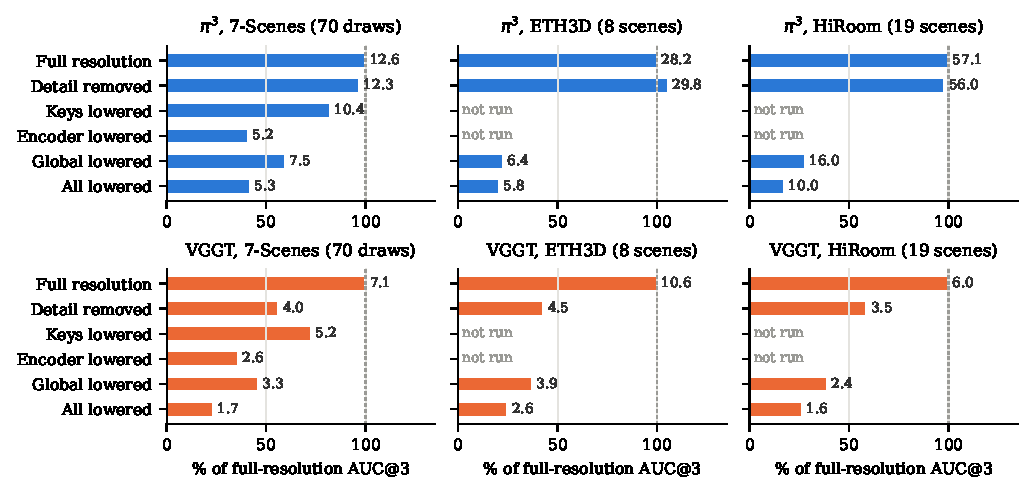
\includegraphics[width=\textwidth]{figures/fig_stages.pdf}
  \caption{\textbf{Every stage we probed needs resolution.} Each bar is the \auc of one probe (\cref{tab:probes}) as a share of the full-resolution input on the same frames; the number beside it is the \auc itself. For \pithree, removing fine pixel detail costs nothing, while lowering the encoder or global attention costs about as much as lowering everything. VGGT loses accuracy under every probe, including removing detail. The encoder and key probes were run on 7-Scenes only.}
  \label{fig:stages}
\end{figure*}

\begin{table}[t]
\centering\small
\setlength{\tabcolsep}{4pt}
\begin{adjustbox}{max width=\linewidth}
\begin{tabular}{@{}lcccc@{}}
\toprule
 & \multicolumn{2}{c}{\pithree} & \multicolumn{2}{c}{VGGT} \\
\cmidrule(lr){2-3}\cmidrule(l){4-5}
Probe (8 of 12 views) & \auc & \aucc & \auc & \aucc \\
\midrule
Full resolution             & 12.6 & 81.9 & 7.1 & 77.8 \\
Detail removed              & 12.3 & 81.4 & 4.0 & 69.7 \\
Encoder lowered             & 5.2  & 70.4 & 2.6 & 66.4 \\
Keys lowered                & 10.4 & 77.4 & 5.2 & 74.5 \\
Global lowered              & 7.5  & 73.0 & 3.3 & 68.5 \\
All lowered                 & 5.3  & 74.5 & 1.7 & 63.2 \\
All lowered, positions not mapped & 1.4 & 51.2 & 0.5 & 31.1 \\
\bottomrule
\end{tabular}
\end{adjustbox}
\caption{\textbf{Stage probes on 7-Scenes} (70 scene-draws). Each row lowers the resolution of the listed stages for 8 of the 12 views (\cref{tab:probes}). Absolute \auc on this dataset is limited by its ground truth (\cref{sec:floor}); \aucc is not.}
\label{tab:stages}
\end{table}

\begin{table}[t]
\centering\small
\setlength{\tabcolsep}{4pt}
\begin{adjustbox}{max width=\linewidth}
\begin{tabular}{@{}lcccc@{}}
\toprule
 & \multicolumn{2}{c}{ETH3D (8 scenes)} & \multicolumn{2}{c}{HiRoom (19 scenes)} \\
\cmidrule(lr){2-3}\cmidrule(l){4-5}
Probe (8 of 12 views) & \pithree & VGGT & \pithree & VGGT \\
\midrule
Full resolution        & 28.2 & 10.6 & 57.1 & 6.0 \\
Detail removed         & 29.8 & 4.5  & 56.0 & 3.5 \\
Global lowered         & 6.4  & 3.9  & 16.0 & 2.4 \\
All lowered            & 5.8  & 2.6  & 10.0 & 1.6 \\
All lowered, not mapped & 1.0 & 0.5  & 1.3  & 0.5 \\
\bottomrule
\end{tabular}
\end{adjustbox}
\caption{\textbf{Stage probes on ETH3D and HiRoom} (pose \auc). Full resolution here is $294{\times}448$ on ETH3D and $364{\times}364$ on HiRoom, which is below VGGT's best size (\cref{fig:response}).}
\label{tab:stages_acc}
\end{table}

\paragraph{The encoder needs full resolution, even for coarse images.}
\emph{Detail removed} and \emph{Encoder lowered} give the network exactly the same image information: both start from the half-resolution image. They differ only in whether the encoder sees that image upsampled to full size or at its own size. For \pithree the difference is large: 12.3 \auc with the full-size encoder against 5.2 with the half-size one, a loss of 7.1 \ci{-8.5}{-5.7}, with the half-size encoder better in only 2 of 70 scene-draws. That loss is about as large as the one from lowering every stage (12.6 to 5.3). Interpolating the encoder's tokens to the full grid does not make up for running the encoder at half resolution. For VGGT the same comparison costs 1.5 \ci{-2.2}{-0.8}.

\paragraph{Global attention needs full resolution too.}
\emph{Global lowered} keeps the pixels, the encoder and frame attention at full resolution and lowers only global attention, together with the heads' view of these 8 views. For \pithree, this alone costs most of what lowering everything costs: 70\% of that loss on 7-Scenes, 97\% on ETH3D (28.2 to 6.4) and 87\% on HiRoom (57.1 to 16.0). Seen the other way, restoring full resolution in the encoder and frame attention while global attention stays at half resolution recovers only 30\%, 2\% and 13\% of the loss on the three datasets. VGGT shows the same pattern at a smaller scale, recovering 29\%, 16\% and 17\%. Resolution is therefore not consumed at a single stage: both the encoder and global attention need it, and full resolution in one cannot make up for its absence in the other.

Mismatched resolution between stages can even hurt coarse accuracy. On ETH3D, \pithree with only global attention lowered reaches 54.8 \aucc, below the 61.6 it reaches with every stage lowered; on 7-Scenes the two are close (73.0 and 74.5). We do not have an explanation for this.

\paragraph{\pithree does not use fine pixel detail; VGGT does.}
Removing the detail above half resolution, while keeping the input size, does not hurt \pithree: its \auc moves from 12.6 to 12.3 on 7-Scenes, rises slightly on ETH3D (from 28.2 to 29.8, a significant $+1.5$, \ci{0.6}{2.6}) and does not change significantly on HiRoom ($-1.1$, \ci{-3.4}{1.1}). VGGT loses accuracy on all three: 3.1 \auc on 7-Scenes, 6.0 on ETH3D \ci{-10.0}{-2.7} and 2.5 on HiRoom \ci{-4.1}{-0.9}.

\paragraph{Positions on a lower-resolution grid must be mapped.}
When a view's tokens sit on a half-resolution grid, its rotary positions describe a smaller image than the full-resolution views'. Mapping them onto the full grid (\cref{eq:align}) is essential: without it, \pithree with every stage lowered drops from 5.3 to 1.4 \auc on 7-Scenes, from 5.8 to 1.0 on ETH3D (a difference of 4.9, \ci{2.8}{7.1}) and from 10.0 to 1.3 on HiRoom, and VGGT loses 2.1 on ETH3D \ci{0.7}{3.7}.

\subsection{Queries and keys in global attention}
\label{sec:keys}

The stage probes leave global attention among the stages that need resolution. This is unwelcome for efficiency, because global attention is the part of the network whose cost grows with the square of the total number of tokens. In attention, though, each token plays two roles: it asks (its query) and it is looked up (its key and value). The two roles need not need the same resolution, so we lower them separately.

Global attention is the stage where views exchange information, and it is the most expensive stage when there are many views. Pooling only the keys and values of the 8 views, while every full-resolution token keeps its own query, costs \pithree 2.3 \auc \ci{-3.6}{-1.0} and VGGT 2.0 \ci{-3.1}{-1.0} on 7-Scenes (\cref{tab:stages}). Starting from the \emph{Detail removed} input instead gives similar losses: 2.2 for \pithree \ci{-3.6}{-0.8} and 2.7 for VGGT \ci{-3.5}{-2.1}. Pooling the queries as well (\emph{Global lowered}) roughly doubles the loss, to 5.1 and 3.9 \auc. For \pithree, pooling keys reduces the transformer compute of these runs by 13\% and pooling queries and keys by 30\%, as estimated from token counts. Queries therefore need full resolution more than keys do, but at 12 views even pooling the keys is not free.

The logit bias that lets a pooled key stand in for the tokens it replaces matters little. Removing it when the encoder is also lowered changes \pithree's \auc by $+0.03$, and adding a similar bias to every lowered view of the \emph{All lowered} probe changes \pithree by $+0.02$ \ci{-0.50}{0.53} and VGGT by $+0.78$ \ci{0.51}{1.06}. How much attention the lowered views receive is thus not the main problem.

\subsection{Errors at different input sizes are correlated}
\label{sec:ensemble}

Every reduction we tried so far costs accuracy, and so does every input size other than a model's best. A remaining hope is that the errors made at different sizes are partly independent, in which case predictions made at several cheap sizes could be combined into one better prediction. We test this on the 70 7-Scenes scene-draws with five uniform input sizes, from $224{\times}294$ to $322{\times}420$. For each pair and triple of sizes, we align the predicted camera sets with a similarity transform, average rotations on SO(3) and camera centres in space, and score the fused poses. Before scoring, we fixed one pair as the test of the idea: the 5{,}184- and 7{,}056-token inputs ($252{\times}336$ and $294{\times}392$). For \pithree, this pair reaches 13.7 \auc, below the 14.4 of the $294{\times}392$ input alone \ci{-1.0}{-0.3}, although it costs more. Across all 20 combinations, every ensemble is significantly worse than the best single size that costs no more, for both models. Only one \pithree ensemble exceeds both of its own members, by 0.3 \auc (12.9 against 12.7 and 12.6). Averaging out a model's error across input sizes therefore does not work, which suggests that most of the error is shared across sizes rather than specific to one.

\subsection{How precise is the benchmark?}
\label{sec:floor}

Throughout these experiments, one dataset behaved differently from the others. Absolute \auc values on 7-Scenes are low for both models (\cref{tab:stages}), and \pithree's response on 7-Scenes is irregular: at uniform sizes from $224{\times}294$ to $322{\times}420$ it scores 9.4, 12.7, 11.7, 14.4 and 12.6, whereas on ETH3D and HiRoom its curve is smooth (\cref{fig:response}). This made us ask how precisely 7-Scenes can measure pose.

We estimated the relative rotation of every pair of views independently, with classical two-view geometry on the full-resolution images: SIFT features, mutual nearest-neighbour matching, and an essential matrix estimated with RANSAC using the dataset's intrinsics. On about 350 pairs with at least 100 inlier matches, the median rotation error against the ground truth is 2.0\textdegree, and only 4\% of these pairs are within 1\textdegree. Changing the assumed focal length from 500 to 620\,px moves this median only between 1.9\textdegree{} and 2.2\textdegree. On the same pairs, \pithree's median error is 1.6\textdegree{} and VGGT's is 1.9\textdegree. Three very different estimators, one of them classical, agree with the ground truth to about the same degree, which points to a limit of the ground truth or its calibration rather than of the methods. We did not establish its cause. Consistent with it, using the classical pair estimates to refine \pithree's poses lowers its \auc on this dataset from 9.4 to 7.9 \ci{-2.3}{-0.7}.

This limit matters for any comparison that relies on \auc on 7-Scenes, since a threshold of 3\textdegree{} is close to the ground truth's own error. We therefore base our response curves on ETH3D and HiRoom, report \aucc alongside \auc, and check the stage findings on all three datasets.
